\documentclass[a4paper]{oblivoir}

\title{쟤료공학개론 과제11}
\author{2018-12432, Electrical and Computer Engineering department, ParkJeonghyun}
\date{12/3/2023}

\newcommand{\be}{\begin{equation}}
\newcommand{\ee}{\end{equation}}

\usepackage{fapapersize}
\usepackage{amsmath}
\usepackage{MnSymbol}
\usepackage{wasysym}
\usepackage{graphicx}
\usepackage{caption}
\usepackage{subfig}
\usepackage{hyperref}
\usepackage{cite}
\usepackage{dtk-logos}
\usepackage{physics}
\usepackage{tikz}
\usetikzlibrary{decorations.markings, positioning}
\usepackage{dtk-logos}
\usepackage{fancyvrb}
\usepackage{array} 
\usepackage{chemformula}

\usefapapersize{ 210mm, 297mm, 15mm, 15mm, 15mm, 15mm}
\DeclareGraphicsExtensions{.pdf, .png, .jpg}

\renewcommand{\figurename}{Figure}

\begin{document}

\maketitle
\section{Problem 1}
A는 아래의 식을 만족한다.
\begin{align}
	A &= \frac{C_{v}}{T^{3}}\\
	&= \frac{12\pi^{4}R}{5\theta_{D}^{3}}
\end{align}
따라서 $\theta_{D}$는 아래의 식을 만족한다.
\begin{align}
	\theta_{D} &= \Bigg(\frac{12\pi^{4}RT^{3}}{5C_{v}}\Bigg)^{1/3}\\
	&= \Bigg(\frac{12\pi^{4}\times 8.3145 \times 15^{3}}{5\times 4.60\times 26.98\times 10^{-3}}\Bigg)^{1/3}\\
	&= 375 K
\end{align}

\section{Problem 2}
\subsection{a}
\begin{align}
	\alpha_{v} &= 3\alpha_{1}\\
	&= 3 \times 14.2 \times 10^{-6 o}C\\
	&= 42.6 \times 10^{-6 o}C
\end{align}

\begin{align}
	\rho &= \frac{\rho_{0}}{1+\alpha_{v}\Delta T}\\
	&= \frac{19.320}{1+42.6 \times 10^{-6} \times (800-20)}g/cm^{3}\\
	&= 18.699 [g/cm^{3}]
\end{align}

\subsection{b}
단위 부피당 원자들의 갯수는 아래와 같다.
\begin{align}
	N &= \frac{6.02\times10^{23}\times 19.320}{26.98}\\
	&= 4.31\times 10^{23}/cm^{3}
\end{align}
따라서 vacancies의 숫자는 아래와 같다.
\begin{align}
	N' &= N \exp(-\frac{E_{v}}{kT})\\
	&= 4.31\times 10^{23}/cm^{3} \times \exp(-\frac{0.98 \times 1.602\times 10^{-19}}{1.38\times 10^{-23} \times (273.15 + 800)})\\
	&= 1.07275 \times 10^{19}cm^{-3}
\end{align}
금은 FCC구조로 한 unit cell에 4개의 원자가 점유하므로 unit cell의 부피는 아래와 같다.
\begin{align}
	V &= \frac{4\times 26.98}{18.699\times 6.02 \times 10^{23}}cm^{3}\\
	&= 9.58710\times 10^{-24}cm^{3}
\end{align}
이 때 단위 격자당 vacancy의 숫자는 unit cell의 부피와 vacancy의 밀도를 곱한 것과 같으므로
\begin{align}
	n' &= 1.07275 \times 10^{19}cm^{-3} \times 9.58710\times 10^{-24}cm^{3}\\
	&= 1.02846\times 10^{-4}
\end{align}
따라서 FCC격자에서 unit cell에 포함되어 있는 4개의 원자들에서 해당 갯수만큼 빠진 원자들이 존재하게 된다. 이를 통해 밀도는 아래와 같이 계산된다.
\begin{align}
	\rho &= \frac{(4- 1.02846\times 10^{-4}) \times 26.98}{6.02 \times 10^{23} \times 9.58710\times 10^{-24}} g / cm^{3}\\
	&= 18.699g / cm^{3}
\end{align}
따라서 변화가 거의 없다

\section{Problem 3}
\subsection{a}
Pure silver가 더 높은 thermal conductivity를 가진다. sterling silver는 혼합물이므로 impurity에 의한 phonon의 scattering이 더 많이 발생할 것이기 때문이다.

\subsection{b}
Fused silica는 여러 상의 실리콘이 결합되어 있으므로 domain으로만 나누어진 poly crystalline silica보다 낮은 thermal conductivity를 가질 것이다. 따라서 polycrystalline silica의 thermal conductivity가 더 크다.

\subsection{c}
Linear and syndiotactic poly(vinyl chloride)가 벤젠구조를 가져 격자간 간격이 더 크므로 phonon의 전파속도가 더 커 열전도율이 더 클 것이다.

\subsection{d}
Atactic polypropylene은 random하게 분자의 광학 성질이 바뀌어 scattering이 발생하므로 isotactic polypropylene이 더 높은 열전도율을 가질 것이다.

\section{Problem 4}
\subsection{a}
열평형에 도달하는데 도달하는 relaxation time은 유한하므로 내부, 외부 사이에 온도차가 발생하게 되고 이로 인해 각각이 평형에 도달했을 때 서로 다른 밀도를 가지므로 응력이 발생한다.

\subsection{b}
냉각시 내부가 더 뜨거우므로 인장 응력이 발생한다.

\subsection{c}
가열시 내부가 더 차가우므로 압축 응력이 발생한다.

%\begin{figure}[htbp]
%	\begin{centering}
%	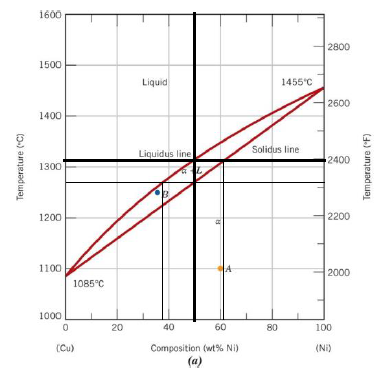
\includegraphics[width = 0.75\linewidth]{pro1.png}% Here is how to import EPS art
%	\caption{\label{fig:pro1} \ch{Ni-Co} Phase Diagram}
%	\end{centering}
%\end{figure}

\end{document}